\documentclass{assignmeownt}
\usepackage{listings}
\usepackage{amsmath}
\usepackage{nccmath}

\DeclareMathOperator*{\argmax}{arg\,max}
\DeclareMathOperator*{\argmin}{arg\,min}


\coursenumber{05124265}
\coursetitle{Reinforcement Learning}
\title{Exercise 2}
\author{Tal Grossman, 201512282 , Moshe Yelisevitch, 207423104}
\date{24/06/2024}


\begin{document}
\maketitle
\thispagestyle{firststyle}
\section{Theory}
\subsection{Question 1}
please see attached PDF file \textbf{Q1.pdf}

\subsection{Question 2}
\begin{enumerate} % Question 2
\item Formal MDP definition:
\newline
\begin{itemize} % question 2 items

\item State space
S = $\{(\nu_0, \dots, \nu_{N}, k) : \nu_i \in \{0, 1\}, k \in \{0, 1,  \dots, 9\}\}$
\newline
Each state is represented by a binary vector of length N+1 and a number k. The "ON" bits in the vecotrs represent the available digits and the number k represent the last random index position.
\newline

\item Action space
A = $\{0, 1, \dots, N\}$
\newline
Possibles actions represents the selection of the index of the next digit. These actions depends on the state space and its current binary vector.
\newline
I.e. the binary vector holds the available positions where the digit can be placed, And so for some vector V, possible actions are: $A(S(V, k)) = \{i : \nu_i = 1\}$

\item Transition probabilities
\newline
$$
P(s' | s, a) = P(\nu_0', \dots, \nu_{N}', k' | \nu_0, \dots, \nu_{N}, k, a) = 
\begin{cases} 
\frac{1}{10} &  a \in A(S(V, k)), \nu_{a}'=0, \nu_{i}'=\nu_{i} : \forall{i}\neq{a},\ k \in\{0, \dots, 9\}   \\
0 & \text{otherwise}
\end{cases}
$$
\newline
The transition probability limits the index selection to the available positions in the binary vector. The probability of the next digit is uniform with an equal probability of $\frac{1}{10}$.

\item Reward function $r(s, a)$ = $r((\nu_0, \dots, \nu_{N}, k), a)$ = $ k \cdot{10^a} $
\newline
the reward is determined by the last index position and the value of the digit in that position.

\item initial state $s_0 = (\{0\}^{N+1}, k): k \in \{0, 1, \dots, 9\} \, each \, w.p \, \frac{1}{10}$
\newline
The initial state is a random number k and a binary vector of length N+1 with all zeros.
\item discount factor $\gamma = 1$
\newline
The discount parameter is set to 1, meaning that the agent does not discount future rewards (Finite horizon problem).

\end{itemize} % question 2 items

\item Optimal policy
\newline
We will prove using induction that the optimal policy depends only on the number of empty slots.
\newline
first, we will proove it holds when there are exactly 2 empty slots, then we will show that if it holds for k empty slots, it holds for k+1 empty slots, thus true for all N+1.
\newline
\underline{Base case:} $k=2$: Assuming the empty cells are $\alpha$ and $\beta$, where $\alpha > \beta$ and the digit is $d$, 
\newline i.e. the state is $s=((0, \dots, \underbrace{1}_{{\alpha}}, \dots, \underbrace{1}_{{\beta}}, \dots, 0), d)$. Now we have 2 possible actions, and \newline
\begin{equation}
    \begin{aligned}
        V(s) &= \max_{a \in A} \left\{ r(s, a) + \sum_{s'} P(s' \mid s, a) V(s') \right\} \\
        &= \max \Biggl( d \cdot 10^{\alpha} + \frac{1}{10} \sum_{i=0}^{9} V((0, \dots, \underbrace{1}_{\beta}, \dots, 0), i), \,
        d \cdot 10^{\beta} + \frac{1}{10} \sum_{i=0}^{9} V((0, \dots, \underbrace{1}_{\alpha}, \dots, 0), i) \Biggr)
    \end{aligned}
\end{equation}
\newline
notice that $ V((0, \dots, \underbrace{1}_{\beta}, \dots, 0), i) = i \cdot 10^{\beta} $ and $ V((0, \dots, \underbrace{1}_{\alpha
}, \dots, 0), i) = i \cdot 10^{\alpha} $.
\newline
now we need to check which is the bigger expression as a function of d, and we get:
\newline
\begin{equation}
    \begin{aligned}
        d \cdot 10^{\alpha} + \frac{1}{10} \sum_{i=0}^{9} i \cdot 10^{\beta} &> d \cdot 10^{\beta} + \frac{1}{10} \sum_{i=0}^{9} i \cdot 10^{\alpha} \\
        \Rightarrow \quad d \cdot 10^{\alpha} + \frac{1}{10} \cdot 10^{\beta} \cdot 45 &> d \cdot 10^{\beta} + \frac{1}{10} \cdot 10^{\alpha} \cdot 45 \\
        \Rightarrow \quad d \cdot (10^{\alpha} - 10^{\beta}) &> 4.5 \cdot (10^{\alpha} - 10^{\beta}) \\
        \Rightarrow \quad d &> 4.5
    \end{aligned}
\end{equation}
\newline
So, if $d > 4.5$ the optimal action is to place the digit in the $\alpha$ position, otherwise in the $\beta$ position.
\newline
\underline{Inductive step:} Assuming the optimal policy depends only on the number of empty slots for k empty slots, we will show that it holds for k+1 empty slots. We'll examin a pair of indices $\alpha$ and $\beta$ where $\alpha > \beta$ and the digit is $d$. I.e. the state is $s=((\nu_0, \dots, \underbrace{1}_{{\alpha}}, \dots, \underbrace{1}_{{\beta}}, \dots, \nu_{N+1}), d)$, such that $\sum_{i=0}^{N} \nu_i = k+1$.
\\
We will show that for every specific pair of indices $\alpha$ and $\beta$, thus its true in general as well.
\\
\underline{for $\alpha$}: $
    d \cdot 10^{\alpha} + \frac{1}{10} \sum_{i=0}^{9} 
    \underbrace{V((\nu_0, \dots, \underbrace{0}_{\alpha}, \dots, \underbrace{1}_{\beta}, \dots, \nu_{N+1})}_{\text{k available slots}}, i) $
\\
\underline{for $\beta$}: $
    d \cdot 10^{\beta} + \frac{1}{10} \sum_{i=0}^{9} 
    \underbrace{V((\nu_0, \dots, \underbrace{1}_{\alpha}, \dots, \underbrace{0}_{\beta}, \dots, \nu_{N+1})}_{\text{k available slots}}, i) $
\\
by the induction hypothesis, both cases are true for k available digits, and true for every pair of indices. 
%% end of question 2.2

%% start of question 2.3
\item optimal policy for $N=2$:
\newline
We will use dynamic programming fir $t=T-1, T-2, \dots, 0$ to find the optimal policy:
\begin{fleqn}
    \begin{equation}
        V(s) = \max_{a \in A}  r(s, a) + \sum_{s' \in S_{t+1}} P(s' \mid s, a) V_{t+1}(s')
    \end{equation}
    \begin{equation}
        \pi^*_t(s) = \argmax_{a \in A}  r(s, a) + \sum_{s' \in S_{t+1}} P(s' \mid s, a) V_{t+1}(s')
    \end{equation}
\end{fleqn}
\\ 
Define $V_3(s) = 0$ where 
\newline
\begin{fleqn}
    \begin{equation}
        V((\nu_0, \nu_1, \nu_2, k), a) = 0 \;\;\; \forall a \in {0, 1, 2}
    \end{equation}
\end{fleqn}
becuase that $\forall i \in {0, 1, 2}, \nu_i = 0$ and no more available slots.
\newline
for $t=2$ we have 1 available slot, and so only one possible action where $\forall k \in \{0, \dots, 9\}$:
\begin{equation}
    \begin{array}{ccc}
        V_2((1, 0, 0, k), 0) = k \cdot 10^0  & V_2((0, 1, 0, k), 1) = k \cdot 10^1 & V_2((0, 0, 1, k), 2) = k \cdot 10^2 \\
        \pi^*_2((1, 0, 0, k)) = 0 & \pi^*_2((0, 1, 0, k)) = 1 & \pi^*_2((0, 0, 1, k)) = 2
    \end{array}
\end{equation}
\newline
for $t=1$ we have 2 available slots, and so 2 possible actions.
\begin{itemize}
    \item{case 1 - slots 1, 2 are available, i.e. $s=(0, 1, 1, k)$:}
    \begin{equation}
        \begin{aligned}
            \pi^*_1((0, 1, 1, k)) = \argmax_{a \in \{2,1\}} \Bigl(
            &r((0, 1, 1, k), 2) + \sum_{s' \in S_2} P((0, 1, 0, k') \mid (0, 1, 1, k), 2) V_2((0, 1, 0, k')) , \\
            &r((0, 1, 1, k), 1) + \sum_{s' \in S_2} P((0, 0, 1, k') \mid (0, 1, 1, k), 1) V_2((0, 0, 1, k'))
            \Bigr) \\ 
            = \argmax_{a \in \{2,1\}} \bigl(
            &k \cdot 10^2 + \frac{1}{10} \sum_{i=0}^{9} i \cdot 10^1,
            k \cdot 10^1 + \frac{1}{10} \sum_{i=0}^{9} i \cdot 10^2
            \bigr) \\
            = \argmax_{a \in \{2,1\}} \bigl(
            &100k + 45, 10k + 450
            \bigr) \\
        \end{aligned}
    \end{equation}
    \newline
    we'll choose action 1 for $s=(0, 1, 1, k)$ when 
    \newline
    \begin{equation}
        100k + 45 \leq 10k + 450 \Rightarrow k \leq 4.5
    \end{equation}
    \newline
    and action 2 otherwise.
    \item{case 2 - slots 0, 1 are available, i.e. $s=(1, 1, 0, k)$:}
    \begin{equation}
        \begin{aligned}
            \pi^*_1((1, 1, 0, k)) = \argmax_{a \in \{1,0\}} \Bigl(
            &r((1, 1, 0, k), 1) + \sum_{s' \in S_2} P((0, 1, 0, k') \mid (1, 1, 0, k), 1) V_2((0, 1, 0, k')) , \\
            &r((1, 1, 0, k), 0) + \sum_{s' \in S_2} P((1, 0, 0, k') \mid (1, 1, 0, k), 0) V_2((1, 0, 0, k'))
            \Bigr) \\ 
            = \argmax_{a \in \{1,0\}} \bigl(
            &k \cdot 10^1 + \frac{1}{10} \sum_{i=0}^{9} i \cdot 10^0,
            k \cdot 10^0 + \frac{1}{10} \sum_{i=0}^{9} i \cdot 10^1
            \bigr) \\
            = \argmax_{a \in \{1,0\}} \bigl(
            &10k + 4.5, k + 45
            \bigr) \\
        \end{aligned}
    \end{equation}
    \newline
    we'll choose action 0 for $s=(1, 1, 0, k)$ when
    \newline
    \begin{equation}
        10k + 4.5 \leq k + 45 \Rightarrow k \leq 4.5
    \end{equation}
    \newline
    and action 1 otherwise.

    \item{case 3 - slots 0, 2 are available, i.e. $s=(1, 0, 1, k)$:}
    \begin{equation}
        \begin{aligned}
            \pi^*_1((1, 0, 1, k)) = \argmax_{a \in \{2,0\}} \Bigl(
            &r((1, 0, 1, k), 2) + \sum_{s' \in S_2} P((0, 0, 1, k') \mid (1, 0, 1, k), 2) V_2((0, 0, 1, k')) , \\
            &r((1, 0, 1, k), 0) + \sum_{s' \in S_2} P((1, 0, 0, k') \mid (1, 0, 1, k), 0) V_2((1, 0, 0, k'))
            \Bigr) \\ 
            = \argmax_{a \in \{2,0\}} \bigl(
            &k \cdot 10^2 + \frac{1}{10} \sum_{i=0}^{9} i \cdot 10^0,
            k \cdot 10^0 + \frac{1}{10} \sum_{i=0}^{9} i \cdot 10^2
            \bigr) \\
            = \argmax_{a \in \{2,0\}} \bigl(
            &100k + 4.5, k + 450
            \bigr) \\
        \end{aligned}
    \end{equation}
    \newline
    we'll choose action 0 for $s=(1, 0, 1, k)$ when
    \newline
    \begin{equation}
        100k + 4.5 \leq k + 450 \Rightarrow k \leq 4.5
    \end{equation}
    \newline
    and action 2 otherwise.
\end{itemize} 

for $t=0$ we have 3 available slots, and so 3 possible actions.
\begin{equation}
    \begin{aligned}
        \pi^*_0((1, 1, 1, k)) = \argmax_{a \in \{0,1,2\}} \Bigl(
        &r((1, 1, 1, k), 0) + \sum_{s' \in S_1} P((0, 1, 1, k') \mid (1, 1, 1, k), 0) V_1((0, 1, 1, k')) , \\
        &r((1, 1, 1, k), 1) + \sum_{s' \in S_1} P((1, 0, 1, k') \mid (1, 1, 1, k), 1) V_1((1, 0, 1, k')) , \\
        &r((1, 1, 1, k), 2) + \sum_{s' \in S_1} P((1, 1, 0, k') \mid (1, 1, 1, k), 2) V_1((1, 1, 0, k'))
        \Bigr) \\ 
        = \argmax_{a \in \{0,1,2\}} \bigl(
        &k + \frac{1}{10} \sum_{i=0}^{4} (10k + 450) + \frac{1}{10} \sum_{i=5}^{9} (100k + 45), \\
        &10k + \frac{1}{10} \sum_{i=0}^{4} (k + 450) + \frac{1}{10} \sum_{i=5}^{9} (100k + 45), \\
        &100k + \frac{1}{10} \sum_{i=0}^{4} (k + 45) + \frac{1}{10} \sum_{i=5}^{9} (10k + 4.5)
        \bigr) \\
        = \argmax_{a \in \{0,1,2\}} \bigl( 
        &k + 607.5, 10k + 578.25, 100k + 60.75
        \bigr) \\
    \end{aligned}
\end{equation}
\newline
we'll choose action 0 for $s=(1, 1, 1, k)$ when
\newline
\begin{equation}
    \begin{array}{cc}
        k + 607.5 \geq 10k + 578.25 \text{ and } k + 607.5 \geq 100k + 60.75 \\
        29.25 \geq 9k \text{ and } 546.75 \geq 99k \\
        k \leq 3.25 \text{ and } k \leq 5.5
    \end{array}
\end{equation}
\newline
we'll choose action 1 for $s=(1, 1, 1, k)$ when
\newline
\begin{equation}
    \begin{array}{cc}
        10k + 578.25 \geq k + 607.5 \text{ and } 10k + 578.25 \geq 100k + 60.75 \\
        9k \geq 29.25 \text{ and } 517.5 \geq 90k \\
        k \geq 3.25 \text{ and } k \leq 5.75
    \end{array}
\end{equation}

we'll choose action 2 for $s=(1, 1, 1, k)$ when
\newline
\begin{equation}
    \begin{array}{cc}
        100k + 60.75 \geq k + 607.5 \text{ and } 100k + 60.75 \geq 10k + 578.25 \\
        99k \geq 546.75 \text{ and } 90k \geq 517.5 \\
        k \geq 5.5 \text{ and } k \geq 5.75
    \end{array}
\end{equation}

\textbf{In Total} for state $s=(1, 1, 1, k)$ the optimal policy is:
\begin{equation}
\pi^*_0((1, 1, 1, k)) = 
\begin{cases}
0 & 0 \leq k \leq 3 \\
1 & 4 \leq k \leq 5 \\
2 & 6 \leq k \leq 9
\end{cases}
\end{equation}
\qedsymbol{}


\end{enumerate} % Question 2

\section{Programming}

\subsection{Question 1: Value Iteration}
TODO-Moshe

\subsection{Question 2: Policy Iteration}
completed in python in the attached file \textbf{policy\_iter.py}
\newline
algorithm policy iteration output:
\begin{figure}[H]
    \centering
    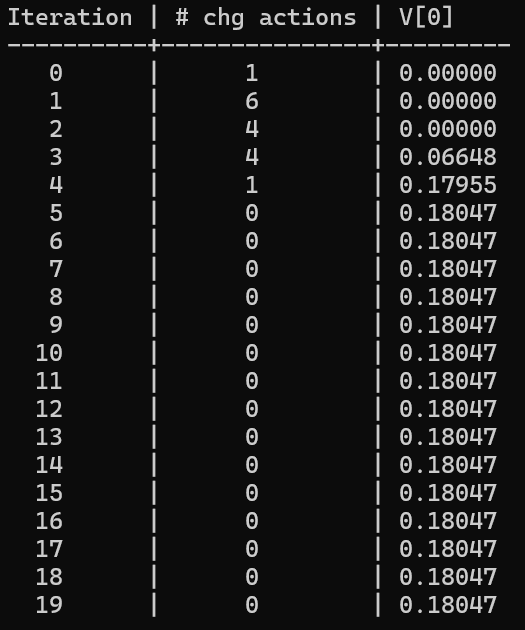
\includegraphics[width=0.3\textwidth]{q2_2_iter_table_print.png}
\end{figure}

\begin{figure}[H]
    \centering
    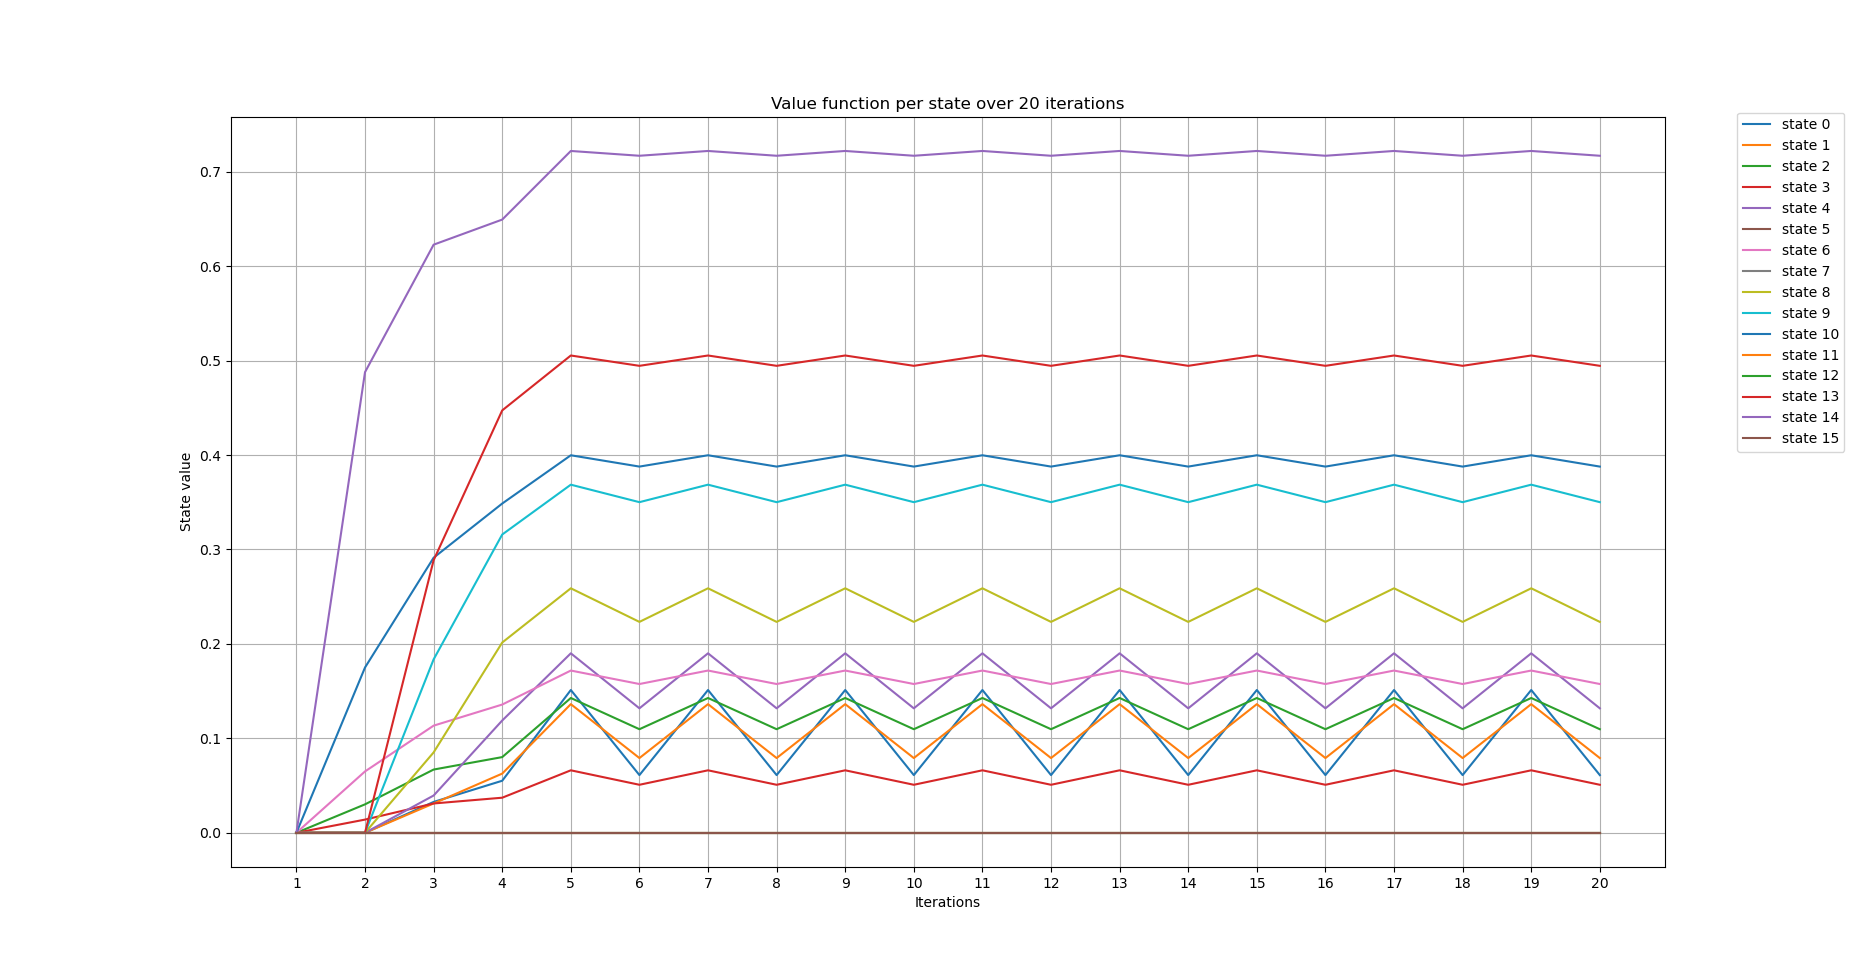
\includegraphics[width=1.0\textwidth]{q2_2_state_value_per_iter_plot.png}
\end{figure}



\end{document}
